\documentclass[conference]{IEEEtran}

\IEEEoverridecommandlockouts

\usepackage{amsmath,amssymb}
\usepackage{booktabs}
\usepackage{cite}
\usepackage[T1]{fontenc}
\usepackage{mathptmx}  % IEEE requires Times; the class asks for ptm but sets
                       % no math family, which leaves math in Computer Modern.
\usepackage{graphicx}
\usepackage{microtype}
\usepackage[dvipsnames]{xcolor}
\usepackage{tikz}
\usepackage{url}
\usetikzlibrary{arrows.meta,fit,positioning}

% ---------------------------------------------------------------------------
% Placeholder macro. Every unresolved item in this manuscript is marked with
% \TODO{...} and states which measurement would close it. Grep for "\TODO{".
% ---------------------------------------------------------------------------
\newcommand{\TODO}[1]{\textcolor{red}{\textbf{[TODO: #1]}}}

% ICRA 2027 uses an eight-page, double-column, double-anonymous submission
% format (references included). Author block is intentionally absent.

% ALT subtitle (if the isolation result turns out weak/ambiguous):
%   ... : What Fixed-Function Offloading Costs and What It Returns
% ALT subtitle: ... : Admissibility, Energy, and GPU Isolation on Jetson Orin
\title{You Only Look Once, Elsewhere: Fixed-Function Perception Offloading
for Energy and GPU Availability in Embedded Robots}

\author{\IEEEauthorblockN{Anonymous Submission}\\
\IEEEauthorblockA{Paper under double-anonymous review}}

\begin{document}
\maketitle

\begin{abstract}
Perception rarely runs alone on a robot: it shares one system-on-chip with
mapping, planning, and control. A fixed-function accelerator such as the NVIDIA
Deep Learning Accelerator (DLA) can host the perception graph and leave the GPU
to the rest of the system, but only if the \emph{entire} learned graph satisfies
its execution contract over operators, tensor rank, layout, and precision. We
therefore treat offloading itself as the decision to be evaluated, and ask what
it costs and what it returns. We retrofit YOLO11n into YOLO11-DLA-n by
substituting exactly two subgraphs, its attention block and its decoded output
interface, and keeping everything else. The retrofit is admissible: TensorRT
compiles it into a single DLA loadable with no layer assigned to the GPU,
whereas the unmodified detector is rejected at its attention matrix
multiplication. Admission is not free. At batch one and $640\times640$ the
strict DLA engine takes $27.515$~ms median engine-plus-transfer time against
$3.740$~ms for the same detector's GPU engine, a factor of $7.36$, and the
retrofit gives up $1.72$ points of COCO $\mathrm{mAP}_{50\text{--}95}$
($37.68$ versus $39.40$, i.e.\ $95.6\%$ retention). Partial offloading is not a
middle ground: with GPU fallback enabled the unmodified detector splits into
four DLA loadables, eleven GPU kernels, and 22 reformat nodes, spends $94.0\%$
of engine time on DLA, and is still slower ($34.678$~ms) than either fully
placed alternative. In a single-threaded reference pipeline the strict path
measures $56.497$~ms end-to-end against $19.203$~ms for the GPU baseline, of
which $13.992$~ms is DLA-native layout packing and unpacking that is an
artifact of the reference implementation rather than of the accelerator. The
offloading decision therefore rests on what strict placement returns in energy
per frame and in GPU availability under contention: \TODO{energy and isolation
results, Sec.~V-E; requires board-power logging across power modes and the
concurrent-workload experiment}.
\end{abstract}

\begin{IEEEkeywords}
Deep learning for visual perception, embedded systems for robotics and
automation, software--hardware integration for robot systems, computer
architecture for robotics and automation, object detection.
\end{IEEEkeywords}

\section{Introduction}
\label{sec:introduction}

A mobile robot runs perception next to mapping, planning, control, and logging,
usually on a single system-on-chip. Whichever processor perception occupies is
not available to the rest of the stack while it is busy, and whatever it draws
comes out of the same power budget. Embedded platforms therefore ship
fixed-function neural accelerators next to the GPU: on NVIDIA Jetson Orin
modules, up to two Deep Learning Accelerator (DLA) cores, depending on the SKU. Their appeal to a robot
integrator is not peak throughput; it is that a detector placed on one of them
stops competing for the GPU and, being fixed-function, is expected to convert
each frame into less energy than a general-purpose engine does.

The obstacle is that such an accelerator does not execute an arbitrary graph. It
implements an execution contract: a set of supported operators plus constraints
on tensor rank, layout, static shapes, precision, kernel parameters, and
dataflow. Regions that violate the contract either fail compilation or, if the
toolchain permits fallback, migrate to the shared processor, which reintroduces
exactly the contention the offload was meant to remove. Hardware support is
consequently not an exporter setting but a property of the model graph.

This paper studies the resulting decision as a systems question with a
measurable price. We take a strong reference detector, YOLO11n
\cite{jocher2024yolo11}, make it admissible with the smallest substitution we
could find that removes every contract violation, and then quantify what the
move to a fixed-function accelerator costs at the engine boundary, at the
application boundary, and in accuracy, so that the energy and availability
benefit can be weighed against a known price rather than assumed. The retrofit,
\emph{YOLO11-DLA-n}, keeps the YOLO11 stem, all C3k2 stages, SPPF, the complete
path-aggregation neck, the head towers, the losses, and the assignment rule, and
replaces two things only: the position-sensitive attention block, whose matrix
multiplications the contract forbids, and the decoded output interface, whose
rank-three anchor decode drags otherwise admissible producers off the
accelerator.

Stating the price plainly is the point of the paper, so we state it here. On the
target module, the strict DLA engine of the retrofit runs at $27.515$~ms median
engine-plus-transfer latency at batch one and $640\times640$, against $3.740$~ms
for the unmodified detector's GPU engine: fixed-function placement is
$7.36\times$ slower at the engine boundary, not faster. The substitution also
costs $1.72$ points of COCO $\mathrm{mAP}_{50\text{--}95}$. Neither number is a
result to be optimized away in this paper; together they are the price of
admission, and our claim is that in a power-capped robot whose GPU is
oversubscribed the price can be repaid in energy per frame and in restored GPU
availability.

Two intermediate positions deserve to be closed off early. The first is partial
offloading. TensorRT can place what it can on DLA and run the rest on the GPU;
for the unmodified detector this produces four DLA loadables, eleven GPU compute
kernels, and 22 reformat nodes, spends $94.0\%$ of engine time on DLA, and is
still slower than the fully placed retrofit and far slower than the GPU engine.
Fallback builds are useful as diagnostics and useless as deployments, so we
report the fallback build only in that role. The second is the temptation to
present accuracy retention as the contribution. Retaining $95.6\%$ of the
reference $\mathrm{mAP}_{50\text{--}95}$ is what makes the offload
\emph{admissible as a perception module at all}; it is a precondition, not a
finding, and we treat it as such.

The contributions are:
\begin{itemize}
  \item a formulation of fixed-function perception offloading as an
  admissibility problem over a declared hardware execution contract, with the
  learned graph separated from variable-cardinality task logic at an explicit
  accelerator boundary;
  \item a minimal admissible retrofit of a current one-stage detector under the
  NVIDIA DLA contract, with a weight-aware initialization that transfers the
  reference model's projections into the substituted block;
  \item a measured price of admission on the target module: strict-build
  acceptance, engine-boundary latency and throughput, accuracy retention, and a
  stage-resolved application-level accounting that separates the accelerator's
  cost from the reference implementation's cost; and
  \item evidence that partial offloading does not provide a compromise, plus the
  protocol and instrumentation for the energy and GPU-isolation measurements on
  which the decision ultimately rests.
\end{itemize}

Hereafter DLA denotes NVIDIA's accelerator, not the homonymous Deep Layer
Aggregation architecture.

\section{Related Work}
\label{sec:related}

\paragraph*{Hardware-aware model design}
Hardware-aware architecture search replaces complexity proxies with objectives
measured on a target platform. MnasNet and ProxylessNAS place measured or
predicted latency inside architecture selection
\cite{tan2019mnasnet,cai2019proxyless}, Once-for-All amortizes specialization
over many deployment constraints \cite{cai2020ofa}, and MCUNet co-designs its
search space with the inference runtime around device memory and operator limits
\cite{lin2020mcunet}. These methods optimize \emph{within} a design space that
is assumed to be executable. The question here precedes them: whether a given
graph is admissible at all under a fixed-function contract, and what the cheapest
edit that makes it admissible costs. Once admissibility is treated as a hard
constraint rather than an objective term, search is the natural follow-up and not
a substitute.

\paragraph*{Real-time and embedded detection}
YOLO formulates detection as dense prediction in a single network
\cite{redmon2016yolo}; later systems advance the real-time frontier with
efficient backbones, multi-scale fusion, better assignment, and end-to-end
prediction \cite{wang2023yolov7,wang2024yolov10}, and YOLO-ReT adapts feature
interaction for edge GPUs \cite{ganesh2022yoloret}. Ultralytics YOLO11
\cite{jocher2024yolo11} is our reference: C3k2 blocks, a path-aggregation neck,
position-sensitive attention, and distributional box regression
\cite{li2020gfl}. Its modularity is what makes a localized, weight-preserving
substitution possible, and its accuracy is what makes the retained accuracy
meaningful. Our independent variable is not the accuracy--latency frontier on a
GPU but the placement of the graph on a different class of processor.

\paragraph*{Accelerator deployment and graph compilers}
TensorRT can assign supported layers to DLA and optionally run the remainder on
the GPU \cite{nvidia_dla_build}; the documented restrictions cover precision,
tensor dimensions, convolution, resize, concatenation, slice, activation, and
softmax \cite{nvidia_dla_working,nvidia_dla_restrictions}. Graph compilers such
as TVM fuse operators and lower networks onto hardware-specific primitives
\cite{chen2018tvm}, but compilation cannot make an inadmissible operator
admissible, which is why we use fallback-free compilation as an acceptance test
rather than as an optimization target. On the model side, the substitution we
need is a spatial mixer without matrix multiplication; external attention shows
that pairwise spatial affinity can be replaced by learned projections through a
compact memory \cite{guo2023external}, and we adopt that idea in the narrow form
that preserves the reference block's interface and residual structure so that
pretrained weights remain usable.

\section{Method}
\label{sec:method}

\begin{figure}[t]
\centering
\resizebox{\columnwidth}{!}{%
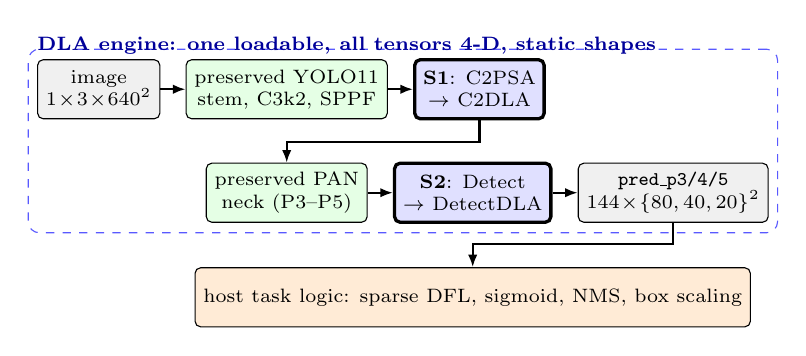
\begin{tikzpicture}[
    node distance=2.6mm and 3.2mm,
    box/.style={draw, rounded corners=2pt, align=center, minimum height=7.5mm,
                inner xsep=3pt, font=\scriptsize},
    kept/.style={box, fill=green!10},
    sub/.style={box, fill=blue!12, very thick},
    io/.style={box, fill=gray!12},
    host/.style={box, fill=orange!16},
    ar/.style={-{Latex[length=1.6mm]}, thick}
]
\node[io] (img) {image\\$1\!\times\!3\!\times\!640^2$};
\node[kept, right=of img] (bb) {preserved YOLO11\\stem, C3k2, SPPF};
\node[sub, right=of bb] (mix)
  {\textbf{S1}: C2PSA\\$\rightarrow$ C2DLA};
\node[kept, below=5.5mm of bb] (neck) {preserved PAN\\neck (P3--P5)};
\node[sub, right=of neck] (head) {\textbf{S2}: Detect\\$\rightarrow$ DetectDLA};
\node[io, right=of head] (maps) {\texttt{pred\_p3/4/5}\\$144\!\times\!\{80,40,20\}^2$};
\node[host, below=5.5mm of head] (post)
  {host task logic: sparse DFL, sigmoid, NMS, box scaling};

\draw[ar] (img) -- (bb);
\draw[ar] (bb) -- (mix);
\draw[ar] (mix.south) -- ++(0,-2.7mm) -| (neck.north);
\draw[ar] (neck) -- (head);
\draw[ar] (head) -- (maps);
\draw[ar] (maps.south) -- ++(0,-2.7mm) -| (post.north);

\node[draw=blue!65, dashed, rounded corners,
      fit=(img)(bb)(mix)(neck)(head)(maps), inner sep=3.2pt] (engine) {};
\node[font=\scriptsize\bfseries, blue!60!black, above=0.4mm of engine.north west,
      anchor=west] {DLA engine: one loadable, all tensors 4-D, static shapes};
\end{tikzpicture}%
}
\caption{Accelerator boundary and the two substitutions. Everything inside the
dashed region compiles to a single DLA loadable; everything outside it is
variable-cardinality task logic that stays on the host. S1 removes the
attention matrix multiplications, S2 removes the rank-three decoded output
interface. Green blocks are inherited from the reference model unchanged.}
\label{fig:boundary}
\end{figure}


\subsection{Execution Contract and Admissibility}
\label{sec:contract}

Let $G=(V,E)$ be a learned perception graph and let
$\mathcal{H}=(\mathcal{O},\mathcal{C})$ be a hardware execution contract:
$\mathcal{O}$ is the supported operator set and $\mathcal{C}$ collects the
configuration constraints, that is tensor rank, layout, static dimensions,
precision, kernel parameter ranges, and admissible dataflow. Write
$A_{\mathcal{H}}(G)=1$ when \emph{every} node of the learned graph is
admissible, the test being supplied by the target compiler rather than by
inspection of the source model. Offloading a detector onto a fixed-function
accelerator is then the problem of obtaining an admissible graph that stays as
close as possible to a reference $G_0$ with function $f_0$, which we treat as a
Pareto problem over structural change and behavioral deviation,
\begin{equation}
\min_{G_R}\ \left(d_{\mathrm{arch}}(G_0,G_R),\,
D_{\mathrm{ref}}(f_0,f_R)\right)
\quad\text{s.t.}\quad A_{\mathcal{H}}(G_R)=1,
\label{eq:retrofit}
\end{equation}
where $d_{\mathrm{arch}}$ measures structural change and $D_{\mathrm{ref}}$
measures deviation under the task metrics and, where required, output agreement
on representative inputs. Equation~\eqref{eq:retrofit} is a design-selection
criterion, not an additional term in the detector's training loss. Its
constraint is binary and supplied by the toolchain, which is what makes the
formulation transferable: on an NPU, an Edge TPU, or an FPGA toolchain the same
criterion applies with a different $\mathcal{H}$ and a different acceptance
procedure. Here $G_0$ is YOLO11 \cite{jocher2024yolo11} and $\mathcal{H}$ is the
NVIDIA DLA contract \cite{nvidia_dla_restrictions,nvidia_dla_build}, whose
relevant clauses are that tensors be four-dimensional with static shapes, that
no matrix multiplication appear, that slices and concatenations act on rank-four
tensors, and that broadcasts be NCHW-compatible.

\subsection{The Accelerator Boundary}
\label{sec:boundary}

Admissibility is not only a question of which operators appear; it is a question
of where the learned graph is declared to end. A detector's terminal
post-processing is inherently variable in cardinality: the number of surviving
candidates depends on image content, and the standard formulation reaches it by
flattening the pyramid into a rank-three tensor of $8400$ anchors, decoding
distributions, building an anchor grid, and suppressing overlaps. None of that
is admissible under $\mathcal{H}$, and worse, its inadmissibility is
contagious. A compiler that partitions a graph by fusible regions will pull
otherwise admissible producers into the fallback partition that feeds its
rank-changing consumer, which is precisely the failure we characterize in
Sec.~\ref{sec:rq2}.

We therefore fix the boundary at static, raw, multi-scale predictions. The
compiled graph accepts a fixed tensor
$I\in\mathbb{R}^{B\times3\times H\times W}$, keeps every intermediate tensor
four-dimensional, and for each pyramid level $\ell\in\{3,4,5\}$ returns
\begin{equation}
P_\ell=\operatorname{Concat}_{C}(R_\ell,S_\ell)
\in\mathbb{R}^{B\times(4r+n_c)\times H_\ell\times W_\ell},
\label{eq:packed}
\end{equation}
where $R_\ell$ holds four $r$-channel distance predictions, $S_\ell$ holds
$n_c$ class logits, and the concatenation is over channels, which the contract
allows on rank-four tensors. No flattening, cross-scale concatenation, anchor
construction, top-$k$, or non-maximum suppression (NMS) is part of the compiled
graph. The host then restores the scale-wise grids and decodes each side
$q\in\{l,t,r,b\}$ by the distributional expectation
\begin{equation}
\hat d_q=\sum_{j=0}^{r-1}j\,
\frac{\exp(R_{qj})}{\sum_{k=0}^{r-1}\exp(R_{qk})},
\label{eq:dfl}
\end{equation}
converts distances relative to cell centers, multiplies by the pyramid stride,
takes $\sigma(S_\ell)$ as class probabilities, and applies NMS.

This boundary is the load-bearing design decision of the paper, and it has three
consequences that we measure separately. First, it is what makes a single
fallback-free loadable possible at all: with the decode inside the graph, no
amount of operator substitution upstream produces an admissible model. Second,
it moves work off the accelerator, so an engine-boundary comparison against a
conventional detector is not a comparison of equal pipelines, since the
reference model emits one decoded $1\times84\times8400$ tensor while the
retrofit emits three raw maps and pays for their decode on the host; we
therefore report a stage-resolved accounting (Sec.~\ref{sec:rq3}) rather than
engine latency alone. Third, it exposes an interface in an accelerator-native
layout: a fixed-function engine is free to demand a packed input format and to
return channel-vectorized outputs, and the cost of meeting that demand is paid
outside the engine, by the host, in whatever implementation the integrator
supplies. That cost is real, it is large in our reference implementation, and it
is not a property of the accelerator; Sec.~\ref{sec:packing} characterizes it
explicitly.

\subsection{YOLO11-DLA-n}
\label{sec:retrofit}

\begin{figure}[t]
\centering
\resizebox{\columnwidth}{!}{%
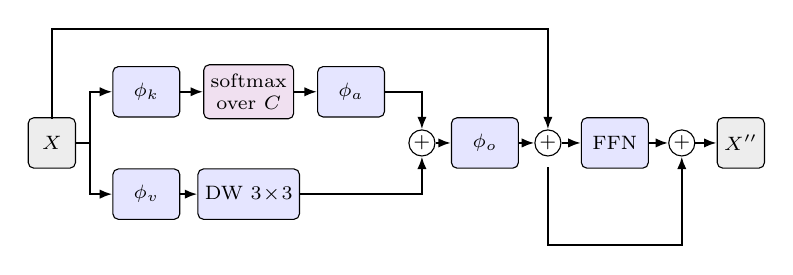
\begin{tikzpicture}[
    op/.style={draw, rounded corners=2pt, align=center, minimum height=6.4mm,
               minimum width=8.5mm, inner xsep=2.5pt, font=\scriptsize},
    conv/.style={op, fill=blue!10},
    act/.style={op, fill=violet!12},
    io/.style={op, fill=gray!14, minimum width=6mm},
    sum/.style={draw, circle, inner sep=0.5pt, font=\scriptsize},
    ar/.style={-{Latex[length=1.6mm]}, thick}
]
\node[io]   at (0.25,-0.65) (b)   {$X$};
\node[conv] at (1.45,0)     (pk)  {$\phi_k$};
\node[act]  at (2.75,0)     (sm)  {softmax\\over $C$};
\node[conv] at (4.05,0)     (pa)  {$\phi_a$};
\node[conv] at (1.45,-1.30) (pv)  {$\phi_v$};
\node[conv] at (2.75,-1.30) (dw)  {DW $3\!\times\!3$};
\node[sum]  at (4.95,-0.65) (s1)  {$+$};
\node[conv] at (5.75,-0.65) (po)  {$\phi_o$};
\node[sum]  at (6.55,-0.65) (r1)  {$+$};
\node[conv] at (7.40,-0.65) (ffn) {FFN};
\node[sum]  at (8.25,-0.65) (r2)  {$+$};
\node[io]   at (9.00,-0.65) (out) {$X''$};

\draw[ar] (b.east) -- ++(0.18,0) |- (pk.west);
\draw[ar] (b.east) -- ++(0.18,0) |- (pv.west);
\draw[ar] (pk) -- (sm);
\draw[ar] (sm) -- (pa);
\draw[ar] (pv) -- (dw);
\draw[ar] (pa.east) -| (s1.north);
\draw[ar] (dw.east) -| (s1.south);
\draw[ar] (s1) -- (po);
\draw[ar] (po) -- (r1);
\draw[ar] (r1) -- (ffn);
\draw[ar] (ffn) -- (r2);
\draw[ar] (r2) -- (out);
% residual around the mixer, Eq. (8)
\draw[ar] (0.25,-0.34) -- (0.25,0.80) -- (6.55,0.80) -- (r1.north);
% residual around the FFN, Eq. (9)
\draw[ar] (6.55,-0.96) -- (6.55,-1.95) -- (8.25,-1.95) -- (r2.south);
\end{tikzpicture}%
}
\caption{One C2DLA mixing block, i.e.\ Eqs.~\eqref{eq:kv}--\eqref{eq:res2}.
Only this branch differs from the reference C2PSA block: the pairwise spatial
attention becomes a rank-$d$ channel-softmax bottleneck built from $1\times1$
convolutions, while the positional depthwise convolution on $V$, both
residuals, and the feed-forward block (two $1\times1$ convolutions with SiLU
between them) are inherited. $X$ is the processed half of the enclosing
split--process--merge structure, which is also inherited; independent $\phi_k$
and $\phi_v$ replace the reference fused QKV projection so that no channel
slice and no shape-helper subgraph reaches the compiler.}
\label{fig:c2dla}
\end{figure}


\subsubsection{Two substitutions}
Under $\mathcal{H}$, exactly two regions of YOLO11n are inadmissible: the
position-sensitive attention in the terminal backbone stage, which forms a
spatial affinity matrix by matrix multiplication, and the decoded output
interface discussed above. The retrofit is therefore
\begin{equation}
\mathrm{C2PSA}\rightarrow\mathrm{C2DLA},\qquad
\mathrm{Detect}\rightarrow\mathrm{DetectDLA},
\label{eq:substitutions}
\end{equation}
and nothing else changes: the stem, all C3k2 stages, SPPF, the full
path-aggregation neck, the channel schedule, the P3--P5 connections, the head
towers, task-aligned one-to-many assignment, the losses, and the $r=16$
distributional regression \cite{li2020gfl} are inherited (Fig.~\ref{fig:boundary},
Table~\ref{tab:design}). What we compare against the reference is thus a
structural approximation of it, not a new detector.

\subsubsection{C2DLA}
C2DLA preserves C2PSA's split--process--merge structure and its residuals, and
replaces only the attention math (Fig.~\ref{fig:c2dla}). Let
$X\in\mathbb{R}^{B\times C\times H\times W}$ be the processed half. One block
computes
\begin{align}
K &= \phi_k(X), \qquad V = \phi_v(X), \label{eq:kv}\\
A_{bkhw} &= \frac{\exp(K_{bkhw})}{\sum_{j=1}^{d}\exp(K_{bjhw})},
  \label{eq:chansoftmax}\\
Z &= \phi_o\!\left(\phi_a(A)+
  \operatorname{DWConv}_{3\times3}(V)\right), \label{eq:mix}\\
X' &= X+Z, \label{eq:res1}\\
X'' &= X'+\phi_2\!\left(\operatorname{SiLU}(\phi_1(X'))\right),
  \label{eq:res2}
\end{align}
with $\phi_k:C\rightarrow d$, $\phi_v:C\rightarrow C$, $\phi_a:d\rightarrow C$
and $\phi_o:C\rightarrow C$ all $1\times1$ convolutions and
$d=\max(C/4,8)$; the unprocessed half and $X''$ are concatenated and projected
as in C2PSA. Three properties matter. The normalization in
\eqref{eq:chansoftmax} runs over channels at each spatial location, so no
affinity matrix and no transpose is formed, and the block follows external
attention in replacing pairwise interaction by projections through a compact
memory of rank $d$ \cite{guo2023external}. The mixing in \eqref{eq:mix} keeps
the reference block's positional depthwise convolution on $V$, which is the
component that supplies local spatial context. Finally, $\phi_k$ and $\phi_v$
are separate convolutions rather than a fused QKV projection followed by a
channel slice: the fused form is equivalent in function but exports as a
\texttt{Slice} chain surrounded by shape helpers, which the compiler places on
the GPU and which then costs a round trip off the accelerator per scale. The
price of the substitution is that mixing is no longer data-dependent or
multi-head; it is a learned low-rank channel mixer gated by a channel softmax.

\subsubsection{DetectDLA}
DetectDLA leaves training untouched: it uses the original box and class towers
and the standard rank-three path in training and in ordinary PyTorch inference.
Only in export mode does it bypass DFL, anchor decoding, sigmoid, and NMS and
emit one packed tensor per scale according to \eqref{eq:packed}. For COCO
($n_c=80$, $r=16$) at $640\times640$ the three engine outputs are
$1\times144\times80\times80$, $1\times144\times40\times40$, and
$1\times144\times20\times20$, exposed as the bindings \texttt{pred\_p3},
\texttt{pred\_p4}, \texttt{pred\_p5} ordered by stride. Export metadata records
the number of raw outputs, the strides, the regression width $r$, the class
names, and whether the head is one-to-one, so that the host decoder is selected
from the engine's declared contract instead of being hard-coded.

\subsubsection{Weight-aware initialization}
Because the edit is localized, most of the reference model transfers directly.
All shape-compatible parameters outside the substituted block are loaded from a
task-matched YOLO11 checkpoint. Inside the block, the positional depthwise
convolution and the output projection are copied verbatim; the per-head
channel slices of the reference fused QKV projection corresponding to $K$ and
$V$, together with their batch-normalization statistics, are gathered into
$\phi_k$ and $\phi_v$ whenever the shapes agree, which for $\phi_k$ requires
$d$ to equal the reference key width; and $\phi_a$, which has no counterpart in
the reference, is initialized randomly. Training then proceeds in two phases:
the layers preceding the substituted block are frozen while the new projection
adapts, after which the whole model is fine-tuned at a lower learning rate.
Initialization is part of the method and not an implementation detail, since it
is what allows a substituted block to approximate a reference block's behavior
rather than merely occupy its position.

\begin{table}[t]
\caption{Reference detector and its admissible retrofit. Only the two rows in
bold differ by construction; every other row is inherited.}
\label{tab:design}
\centering
\scriptsize
\setlength{\tabcolsep}{2.5pt}
\renewcommand{\arraystretch}{1.1}
\begin{tabular}{p{0.20\columnwidth}p{0.34\columnwidth}p{0.36\columnwidth}}
\toprule
Axis & YOLO11n (reference) & YOLO11-DLA-n (retrofit) \\
\midrule
Stem, C3k2 stages, SPPF, PAN neck & inherited & identical \\
\textbf{Terminal backbone stage} & C2PSA, position-sensitive attention with
two matrix multiplications & C2DLA, rank-$d$ channel-softmax mixer, $1\times1$
convolutions only \\
Positional encoding & $3\times3$ depthwise on $V$ & unchanged \\
Activations & SiLU & unchanged \\
Box representation & $r=16$ distributional & unchanged \\
Assignment, losses & task-aligned one-to-many & unchanged \\
\textbf{Exported interface} & one decoded $1\times84\times8400$ tensor &
three raw maps, $4r+n_c=144$ channels per scale \\
Host task logic & NMS & DFL decode, sigmoid, NMS \\
Initialization & official COCO checkpoint & shape-compatible transfer, block
hot-start, two-phase fine-tune \\
Strict DLA build & rejected at the attention \texttt{MatMul} & accepted, one
loadable, no layer on GPU \\
\bottomrule
\end{tabular}
\end{table}

\section{DLA Case-Study Deployment}
\label{sec:deployment}

\subsection{Static Engine Interface}

The model is fused and exported to ONNX with a fixed batch size and input
resolution. TensorRT parses the graph in FP16 and targets DLA core~0 of the
module; the engine exposes one image input and the three stride-ordered
prediction bindings of Sec.~\ref{sec:retrofit}. Because the accelerator is the
default device and fallback is disabled, the compiler either accepts the whole
graph or refuses to build, which is the property we use as an acceptance test.

\subsection{Confidence-First Sparse DFL Decode}

The host decoder splits the first $4r=64$ channels from the $n_c=80$ class
logits at each scale. Since a candidate's class confidence does not depend on
its box distribution, the decoder first discards every anchor whose maximum
class logit falls below the inverse-sigmoid image of the confidence threshold,
$\log\frac{\tau}{1-\tau}$, and only then restores grids and applies the 16-bin
expectation \eqref{eq:dfl} to the survivors, converts distances to boxes,
applies $\sigma(\cdot)$, and runs standard NMS. Up to floating-point roundoff
this is equivalent to dense decoding followed by the same threshold, because
thresholding commutes with a per-anchor box transform that it does not read;
the dense path is retained in the implementation as an equivalence gate and is
the reference against which the sparse path is checked. The saving is large
because the surviving fraction is small: at $\tau=0.25$ on the test image, 13 of
$8400$ anchors survive (Sec.~\ref{sec:rq3}).

\subsection{DLA-Native Input Packing and Output Unpacking}
\label{sec:packing}

The strict engine does not accept a linear NCHW image and does not return
linear NCHW predictions, and this is the single most consequential difference
between deploying on the accelerator and deploying on the GPU. It is built with
\texttt{--inputIOFormats=fp16:dla\_hwc4} and
\texttt{--outputIOFormats=fp16:chw16}, and the build-time layer dump confirms
the input as the DLA image format, ``channel major FP16 where
$C \bmod 4 = 0$'', and the three outputs as ``sixteen wide channel vectorized
row major FP16''. At $640\times640$ the input is a 3-channel image padded to 4
channels and interleaved per pixel, with each row aligned to 64 bytes, giving a
$4\times640\times640$ FP16 buffer of $3.28$~MB; the outputs need no channel
padding, since $144=9\times16$, and total $144\times8400$ FP16 values, i.e.\
$2.42$~MB. \TODO{the runtime-reported binding format string for this engine is
not recorded in our logs; the TensorRT Python API may report a
channel-vectorized alias for the DLA image format, which changes nothing about
the buffer geometry but should be recorded in the final runs}

Where this conversion runs, and in what implementation, is a property of the
integrator and not of the accelerator, so we state it exactly. In our reference
pipeline both directions run \emph{on the host CPU in single-threaded PyTorch}
(\texttt{torch.set\_num\_threads(1)}). Packing allocates a zero-filled padded
tensor, copies a permuted NCHW-to-interleaved view into it, flattens it, and
copies it synchronously into the device buffer; unpacking copies the device
buffer to the host and then applies a view, a permutation, a
\texttt{contiguous()} materialization, and a float cast per output. There is no
CUDA kernel, no pinned staging buffer, no NEON-tuned or vectorized packer, and
no overlap between conversion and execution. This is a deliberately simple
reference implementation, and Sec.~\ref{sec:rq3} reports its cost as such.

\subsection{Compliance Gates}

We instantiate $A_{\mathcal{H}}(G)=1$ as strict DLA execution only if all of the
following hold, in order:
\begin{enumerate}
  \item the model is fused before export, and every engine input and learned
  output has a fixed four-dimensional shape;
  \item the exported ONNX graph contains no rank-changing terminal subgraph, no
  matrix multiplication, and no dynamic shape operator, audited on the graph
  rather than assumed from the exporter flags;
  \item TensorRT builds with DLA as the default device and GPU fallback
  disabled, so that a single inadmissible node is a build failure;
  \item the verbose build log and the engine inspector report no GPU-assigned
  learned layer, apart from unavoidable host-side I/O handling; and
  \item externally decoded predictions agree with the ordinary PyTorch
  inference path within a documented tolerance, and the sparse decoder agrees
  with the dense one.
\end{enumerate}
Gate~2 is an audit of the graph the compiler will see, not a whitelist claim
about the source model: the retrofit inherits a static channel split, a channel
softmax, and SiLU decompositions whose fusion is a compiler behavior that can
change across toolchain versions, so gate~3 remains the binding criterion and
gate~2 exists to explain build failures rather than to predict success. Gates 3
and 4 are evaluated on the target module, because engines and DLA loadables are
specific to the hardware and software stack that produced them. A
fallback-enabled build never satisfies these gates and is reported only as a
diagnostic. On a different accelerator, gates 1, 3, 4, and 5 carry over
verbatim and only the operator audit of gate~2 is replaced.

\section{Evaluation}
\label{sec:eval}

Four research questions organize the evaluation. \textbf{RQ1}: what does making
the graph admissible cost in task accuracy? \textbf{RQ2}: is the retrofit
actually admissible under fallback-free compilation, and what is the latency and
throughput price at the engine boundary? \textbf{RQ3}: how does that price
appear at the application boundary once preprocessing, layout conversion, and
host decoding are accounted for? \textbf{RQ4}: what does strict placement return
in energy per frame and in GPU availability under contention? RQ1--RQ3 are
answered with measurements; RQ4 is specified, instrumented, and not yet
measured, and we mark it as such rather than argue it.

We test one hypothesis, H1: a substitution restricted to the inadmissible
regions of a strong detector, initialized from that detector's weights, retains
most of its accuracy, so that admissibility can be bought at a task cost small
enough to be irrelevant to the deployment decision. The deployment decision
itself is then determined by RQ2--RQ4 and not by H1.

\subsection{Setup}
\label{sec:setup}

\paragraph*{Platform}
All device measurements come from one NVIDIA Jetson Orin module. The build logs
record device name \texttt{Orin}, compute capability $8.7$, 16 streaming
multiprocessors, $62\,840$~MiB of shared device memory, a 256-bit memory bus, an
application compute clock of $1.3$~GHz, TensorRT $10.3.0$, and DLA core~0 with
DLA memory pools of 1~MiB managed SRAM, 1024~MiB local DRAM, and 512~MiB global
DRAM. \TODO{exact module SKU and carrier, JetPack/L4T version, CUDA and cuDNN
versions, active \texttt{nvpmodel} power mode, \texttt{jetson\_clocks} state,
measured GPU/DLA/EMC clocks during each run, and thermal state; none of these
are in the current logs and all must be recorded with the final runs}

\paragraph*{Models and accuracy protocol}
The reference is the official COCO-pretrained YOLO11n checkpoint; the retrofit
is its best validation checkpoint \TODO{exact training schedule of the reported
retrofit checkpoint: epoch budget of each phase and the frozen-adaptation
length; the checkpoint file name in our records suggests a different epoch
count than the one we had noted}. Both are evaluated on the same COCO val2017
split \cite{lin2014coco} at $640\times640$ over the same 80 classes. Precision
and recall are averaged over classes at the confidence operating point that
maximizes mean F1. Reference retention is $100\,Q(G)/Q(G_0)$ with
$Q=\mathrm{mAP}_{50\text{--}95}$.

\paragraph*{Deployment protocol}
Three builds are used: TensorRT GPU FP16 as the primary baseline, TensorRT with
DLA requested and GPU fallback enabled as a partitioning diagnostic, and strict
DLA FP16 with fallback disabled. All comparisons are at FP16, batch one, and
$640\times640$. Engine-boundary numbers come from \texttt{trtexec} with
generated inputs, a 2~s warm-up, a 30~s run, one inference stream, spin waiting,
and H2D and D2H transfers included; TensorRT's reported host latency is the sum
of H2D, device execution, and D2H, and excludes preprocessing and detector
post-processing, so we call it engine-plus-transfer latency and never
end-to-end latency. Application-level numbers come from one instrumented tester
that letterboxes a $960\times1280$ image to $640\times640$ and runs 100 timed
iterations after ten full-pipeline warm-ups, with single-threaded CPU
post-processing, $\tau=0.25$, and NMS IoU $0.45$; file reading, annotation, and
image writing are excluded.

\subsection{RQ1: Accuracy and Retention (the Price of Admission)}
\label{sec:rq1}

Table~\ref{tab:accuracy} reports the model-level comparison. The retrofit
reaches $37.68\%$ $\mathrm{mAP}_{50\text{--}95}$ against $39.40\%$ for the
reference, i.e.\ it gives up $1.72$ points and retains $95.6\%$; precision,
recall, and $\mathrm{mAP}_{50}$ fall by $0.94$, $1.22$, and $1.97$ points. This
supports H1 and closes RQ1: the accuracy cost of removing two inadmissible
subgraphs from a modern detector is under two points of
$\mathrm{mAP}_{50\text{--}95}$, which for most robot deployments is not the
term that decides where the model runs. We deliberately do not present this as
the result of the paper. It is the precondition that makes the rest of the
comparison meaningful, and it is measured on the PyTorch path, not through the
serialized accelerator engine.

\begin{table}[t]
\caption{COCO val2017 detection accuracy at $640\times640$, percent. The first
four columns are measured on the ordinary PyTorch inference path. The last
column, which is what the deployed strict engine actually delivers, is not yet
measured.}
\label{tab:accuracy}
\centering
\scriptsize
\setlength{\tabcolsep}{2.2pt}
\begin{tabular}{lccccc}
\toprule
 & \multicolumn{4}{c}{PyTorch path} & Strict DLA engine \\
\cmidrule(lr){2-5}\cmidrule(lr){6-6}
Model & P & R & $\mathrm{mAP}_{50}$ & $\mathrm{mAP}_{50\text{--}95}$
      & $\mathrm{mAP}_{50\text{--}95}$ \\
\midrule
YOLO11n      & 65.64 & 50.25 & 55.14 & 39.40 & n/a (build rejected) \\
YOLO11-DLA-n & 64.70 & 49.03 & 53.17 & 37.68 & \TODO{measure} \\
\bottomrule
\end{tabular}
\end{table}

The empty cell in Table~\ref{tab:accuracy} is a real gap, not a formality.
\TODO{COCO $\mathrm{mAP}_{50\text{--}95}$ evaluated from the serialized strict
DLA engine. The stock Ultralytics TensorRT backend cannot bind CHW16 outputs or
a DLA image input, so this requires running the validator through the custom
tester path of Sec.~\ref{sec:packing}; FP16 rounding, the compiler's DLA
softmax approximation, and the packing path can all move the number} Until it is
filled, every accuracy statement in this paper describes the PyTorch model and
not the engine.

\subsection{RQ2: Admissibility and the Engine Boundary}
\label{sec:rq2}

\paragraph*{Admissibility}
The unmodified detector is rejected. With DLA as the default device and fallback
disabled, the build aborts at \texttt{/model.10/m/m.0/attn/MatMul} with
\emph{``MatMul is unsupported on DLA''} followed by a DLA validation failure, so
no engine exists to measure. The retrofit is accepted: the verbose build reports
299 layers running on DLA and \emph{``No layer is running on GPU''}, and the
engine inspector represents the whole learned graph as a single \texttt{DLA}
layer with the three declared prediction bindings. Compliance gates 1--4 of
Sec.~\ref{sec:deployment} are therefore satisfied; gate~5 is satisfied at the
level of the interface check reported in Sec.~\ref{sec:rq3} and not yet at the
level of dataset accuracy.

\paragraph*{Why partial offloading is not an option}
The fallback build is the natural compromise a practitioner would try, and it
does not work. TensorRT keeps 317 layers on DLA and moves 17 to the GPU: the two
attention matrix multiplications, eight reshape/transpose shuffles, two slices,
one division, and four constants. The reasons the log gives for the head are
instructive, because they are shape reasons rather than operator reasons:
\emph{``Input tensor has less than 4 dimensions''} and \emph{``Dimension: 3
(8400) exceeds maximum allowed size for DLA: 8192''}. The decoded interface is
inadmissible twice over, once for rank and once for extent, which is what
motivates the boundary of Sec.~\ref{sec:boundary}.

After fusion the resulting engine contains 47 nodes: four DLA loadables, 11 GPU
compute kernels, 22 reformat nodes, seven no-ops, and three constants. The layer
profiler attributes $93.97\%$ of execution time to the four DLA loadables,
$4.73\%$ to the reformat nodes, and $1.31\%$ to all GPU compute together; the
largest single DLA segment, which ends at the attention transpose, accounts for
$42.54\%$ ($14.581$~ms). So the GPU does almost no arithmetic in this build, and
the build is still the slowest of the three at $34.678$~ms median. Coverage
statistics are the wrong metric for a partitioned graph: what costs time is the
partitioning itself, in layout conversion and in serialization of four
loadables. A build that is $94\%$ on the accelerator still holds the GPU, still
pays $22.80$~MiB of execution-context device memory, and its median
engine-plus-transfer latency is $26.0\%$ above that of the fully placed strict
engine. We report it as a diagnostic and not as a
deployment option.

\paragraph*{The price at the engine boundary}
Table~\ref{tab:engine} gives the matrix. The comparison that matters is the
strict engine against the primary baseline, the reference detector on the GPU:
$27.515$~ms against $3.740$~ms median engine-plus-transfer latency, a factor of
$7.36$, and $37.2$ against $288.3$ queries/s saturated throughput, i.e.\
$12.9\%$. Against the retrofit's own GPU engine the factor is $7.86$. Transfers
are not the reason: for the strict engine the median splits into $0.393$~ms
H2D, $26.816$~ms device execution, and $0.305$~ms D2H, so $97.5\%$ of the
engine-boundary time is the accelerator computing. This is what a
fixed-function core costs on this workload, and no boundary placement or
implementation effort inside the engine will remove it.

Two secondary observations. First, the retrofit is not slower than the reference
on the GPU: $3.500$ against $3.740$~ms median and $317.2$ against
$288.3$~queries/s, which is an interface difference rather than an architecture
win, since the retrofit's engine stops before the decode that the reference
performs internally. Second, the strict engine is the cheapest to build and to
hold: $18.7$~s build time against $471.7$~s for the reference GPU engine,
$6.52$~MiB serialized against $8.15$~MiB, and zero execution-context device
memory against $9.47$~MiB, because its activations live in the accelerator's own
memory pools. Those allocator figures support the placement audit; they are not
a substitute for the concurrency measurement of Sec.~\ref{sec:rq4}.

\begin{table}[t]
\caption{FP16 TensorRT engine boundary, batch one, $640\times640$, DLA core~0.
Latency includes H2D, device execution, and D2H, and excludes pre- and
post-processing. DLA share is profiler time, not layer count. Each row is one
30~s \texttt{trtexec} launch.}
\label{tab:engine}
\centering
\scriptsize
\setlength{\tabcolsep}{2.0pt}
\begin{tabular}{lccrrr}
\toprule
Model / execution & Build & DLA & Median & P95 & Thr. \\
                  &       & (\%) & (ms)  & (ms) & (q/s) \\
\midrule
YOLO11n / GPU (baseline)   & yes & 0    & 3.740  & 3.753  & 288.3 \\
YOLO11n / DLA+GPU (diagn.) & yes & 94.0 & 34.678 & 34.942 & 29.2 \\
YOLO11n / strict DLA       & \textbf{no} & --- & --- & --- & --- \\
YOLO11-DLA-n / GPU         & yes & 0    & 3.500  & 3.512  & 317.2 \\
YOLO11-DLA-n / strict DLA  & yes & 100  & 27.515 & 27.718 & 37.2 \\
\bottomrule
\end{tabular}
\end{table}

\subsection{RQ3: Application-Level Accounting}
\label{sec:rq3}

% Stacked per-stage accounting; bar lengths are the median stage times of
% Table~\ref{tab:e2e}. Horizontal unit: 1 ms.
\begin{figure}[t]
\centering
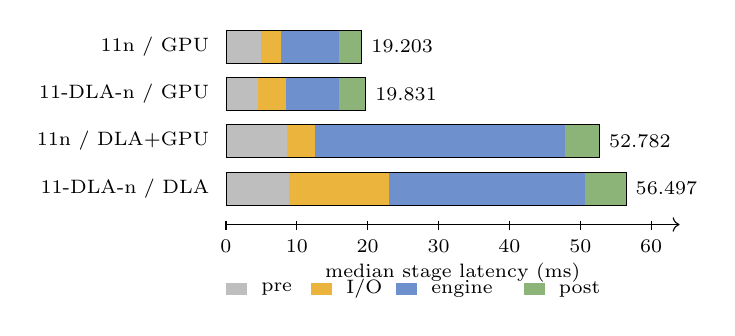
\begin{tikzpicture}[x=0.090cm, y=1cm,
  lab/.style={font=\scriptsize, anchor=east},
  tot/.style={font=\scriptsize, anchor=west}]

\definecolor{cpre}{RGB}{190,190,190}
\definecolor{cio}{RGB}{235,180,60}
\definecolor{ceng}{RGB}{110,145,205}
\definecolor{cpost}{RGB}{140,180,120}

\newcommand{\stackbar}[6]{%
  \node[lab] at (-1,#1+0.21) {#6};
  \fill[cpre]  (0,#1) rectangle (#2,#1+0.42);
  \fill[cio]   (#2,#1) rectangle (#2+#3,#1+0.42);
  \fill[ceng]  (#2+#3,#1) rectangle (#2+#3+#4,#1+0.42);
  \fill[cpost] (#2+#3+#4,#1) rectangle (#2+#3+#4+#5,#1+0.42);
  \draw[very thin] (0,#1) rectangle (#2+#3+#4+#5,#1+0.42);
}

\stackbar{0}{4.900}{2.843}{8.153}{3.250}{11n / GPU}
\node[tot] at (19.15,0.21) {19.203};
\stackbar{-0.60}{4.572}{3.848}{7.560}{3.717}{11-DLA-n / GPU}
\node[tot] at (19.70,-0.39) {19.831};
\stackbar{-1.20}{8.617}{4.002}{35.198}{4.866}{11n / DLA+GPU}
\node[tot] at (52.69,-0.99) {52.782};
\stackbar{-1.80}{8.946}{13.992}{27.788}{5.711}{11-DLA-n / DLA}
\node[tot] at (56.44,-1.59) {56.497};

\draw[->] (0,-2.05) -- (64,-2.05);
\foreach \x in {0,10,20,30,40,50,60}
  {\draw (\x,-2.00) -- (\x,-2.12) node[below, font=\scriptsize] {\x};}
\node[font=\scriptsize, anchor=north] at (32,-2.42) {median stage latency (ms)};

\fill[cpre] (0,-2.95) rectangle (3,-2.79);
\node[font=\scriptsize, anchor=west] at (3.6,-2.87) {pre};
\fill[cio] (12,-2.95) rectangle (15,-2.79);
\node[font=\scriptsize, anchor=west] at (15.6,-2.87) {I/O};
\fill[ceng] (24,-2.95) rectangle (27,-2.79);
\node[font=\scriptsize, anchor=west] at (27.6,-2.87) {engine};
\fill[cpost] (42,-2.95) rectangle (45,-2.79);
\node[font=\scriptsize, anchor=west] at (45.6,-2.87) {post};
\end{tikzpicture}
\caption{Per-stage accounting of the repeated-image pipeline check, reference
implementation, single-threaded CPU pre- and post-processing
(Table~\ref{tab:e2e}). I/O is input packing plus H2D, plus D2H plus output
unpacking. Numbers at the right are median totals; because stage medians are
computed independently they need not sum exactly to the median total. The
strict DLA row is the only one whose I/O stage carries a DLA-native layout
conversion, and the only one whose engine stage uses no GPU.}
\label{fig:stack}
\end{figure}


Table~\ref{tab:e2e} and Fig.~\ref{fig:stack} decompose one instrumented
pipeline over the four configurations that have data. The strict path measures
$56.497$~ms median total against $19.203$~ms for the baseline, a factor of
$2.94$; the sequential image rates are $17.70$ and $52.08$~images/s, which are
inverse median latencies and not saturated throughput. Decomposing the
$37.29$~ms difference by stage is more informative than the ratio: the engine
contributes $+19.64$~ms, layout conversion $+11.15$~ms, preprocessing
$+4.05$~ms, and host decoding $+2.46$~ms.

Only the first of those four terms is intrinsic to the accelerator. The second
is the reference implementation's cost, and we state its nature plainly:
packing the DLA image input and unpacking the three CHW16 outputs together take
$13.992$~ms ($7.755$~ms in, $6.237$~ms out) against $2.843$~ms for the
baseline's linear bindings, for buffers of $3.28$ and $2.42$~MB respectively.
That is an effective conversion rate of roughly $0.42$ and $0.39$~GB/s, far
below the module's memory bandwidth, which is unsurprising for
single-threaded PyTorch tensor permutations on the CPU as described in
Sec.~\ref{sec:packing}. Table~\ref{tab:e2e} is therefore a characterization of
\emph{this reference implementation}, not a measurement of the intrinsic cost of
the DLA path, and the comparison it supports is bounded pending an optimized
converter. \TODO{stage row for an optimized I/O path: a CUDA or NEON packer, a
pinned staging buffer, conversion overlapped with execution, and a decoder that
consumes CHW16 directly; this row is the honest upper bound on how much of the
$11.15$~ms is removable}

The third and fourth terms are not explained by any code path. Preprocessing is
identical OpenCV letterboxing of the identical image in every row, yet it
measures $4.900$ and $4.572$~ms in the two GPU rows and $8.617$ and $8.946$~ms
in the two DLA rows. Host post-processing is likewise the same single-threaded
code on the same 13 surviving anchors for both retrofit rows, yet it measures
$3.717$~ms with the GPU engine and $5.711$~ms with the strict engine. The two
DLA-row processes are thus about $6.4$~ms slower on stages that never touch the
accelerator. We report this as an unexplained cross-process measurement
difference between process launches and decline to attribute it to thermal,
clock, or scheduling effects, none of which we recorded. It bounds the precision
of the totals in Table~\ref{tab:e2e} and is a first-order reason to repeat the
experiment as specified in Sec.~\ref{sec:validity}.

Two further results belong here. The interface check passes: the retrofit's GPU
and strict-DLA executions return the same two detections with the same
confidences (\texttt{person} $0.871$, \texttt{bench} $0.317$) and box
coordinates differing by at most $0.3$~pixels, which validates the packing and
unpacking path for this input without substituting for engine-level dataset
validation. And the confidence-first decoder of Sec.~\ref{sec:deployment} is
what keeps host decoding affordable: it reduces median post-processing from
$17.011$ to $3.717$~ms on the GPU engine and from $26.744$ to $5.711$~ms on the
strict engine, while returning the same detections. Without it, the host decode
alone would exceed the entire baseline pipeline.

\begin{table}[t]
\caption{Repeated-image pipeline check, one process launch per row, medians in
milliseconds; I/O sums input packing/H2D and D2H/unpacking; P95 and P99 refer to
the total. \emph{This is a characterization of the reference implementation}:
pre-, post-processing and layout conversion are single-threaded CPU code that
has not been optimized.}
\label{tab:e2e}
\centering
\scriptsize
\setlength{\tabcolsep}{1.6pt}
\begin{tabular}{lrrrrrrr}
\toprule
Execution & Pre & I/O & Eng. & Post & Total & P95 & P99 \\
\midrule
11n / GPU        & 4.900 & 2.843  & 8.153  & 3.250 & \textbf{19.203} & 19.574 & 19.880 \\
11n / DLA+GPU    & 8.617 & 4.002  & 35.198 & 4.866 & \textbf{52.782} & 53.098 & 53.396 \\
11-DLA-n / GPU   & 4.572 & 3.848  & 7.560  & 3.717 & \textbf{19.831} & 20.343 & 20.544 \\
11-DLA-n / DLA   & 8.946 & 13.992 & 27.788 & 5.711 & \textbf{56.497} & 56.864 & 57.781 \\
\addlinespace
\multicolumn{8}{l}{\emph{optimized I/O bound, same engine:}} \\
11-DLA-n / DLA   & \multicolumn{7}{l}{\TODO{optimized packer}} \\
\bottomrule
\end{tabular}
\end{table}

\subsection{RQ4: Energy and GPU Isolation}
\label{sec:rq4}

\begin{figure}[t]
\centering
\fbox{\parbox[c][3.1cm][c]{0.94\columnwidth}{\centering\footnotesize
\TODO{Fig.~4: GPU isolation. Planned content: latency distribution of a
concurrent CUDA workload run alone and run beside (i) the GPU baseline engine,
(ii) the fallback engine, and (iii) the strict DLA engine, plus the perception
latency distribution in each case. Requires the co-execution experiment of
Sec.~\ref{sec:rq4}; no data collected yet.}}}
\caption{Placeholder for the GPU-isolation result. The offloading decision of
this paper rests on this measurement together with Table~\ref{tab:energy}.}
\label{fig:isolation}
\end{figure}


RQ1--RQ3 establish the price: $1.72$ points of $\mathrm{mAP}_{50\text{--}95}$,
$7.36\times$ engine-boundary latency, and, in the current reference pipeline,
$2.94\times$ application latency. The paper's claim is that this price is
repaid in two currencies that matter on a power-capped robot with an
oversubscribed GPU, and this subsection is where that claim is tested. It is
not yet tested. We give the protocol, the instrumentation, and the table
skeleton, and mark every cell that requires data.

\paragraph*{Energy per frame}
Board power is logged after thermal stabilization in a fixed power mode, at
batch one, on the ordered image set, with the pipeline saturated and with it
running at a fixed frame rate; both total board energy per frame and
idle-subtracted energy per frame are retained, since the idle draw of the rest
of the module is not attributable to perception. The comparison of interest is
the strict engine against the GPU baseline at equal delivered frame rate, not at
equal utilization, because a robot's camera rate is fixed and the question is
what each placement costs per frame at that rate. Table~\ref{tab:energy} is the
intended form.

\begin{table}[t]
\caption{Energy accounting. Every cell requires the board-power measurement
described in Sec.~\ref{sec:rq4}; no energy data has been collected.}
\label{tab:energy}
\centering
\scriptsize
\setlength{\tabcolsep}{2.2pt}
\begin{tabular}{llccc}
\toprule
Power mode & Execution & Mean board & $E$/frame & $E$/frame \\
           &           & power (W)  & (mJ)      & idle-sub. (mJ) \\
\midrule
\TODO{mode A} & 11n / GPU       & \TODO{} & \TODO{} & \TODO{} \\
              & 11n / DLA+GPU   & \TODO{} & \TODO{} & \TODO{} \\
              & 11-DLA-n / DLA  & \TODO{} & \TODO{} & \TODO{} \\
\addlinespace
\TODO{mode B} & 11n / GPU       & \TODO{} & \TODO{} & \TODO{} \\
              & 11n / DLA+GPU   & \TODO{} & \TODO{} & \TODO{} \\
              & 11-DLA-n / DLA  & \TODO{} & \TODO{} & \TODO{} \\
\bottomrule
\end{tabular}
\end{table}

\paragraph*{GPU availability under contention}
Isolation is measured at two levels. First, a controlled CUDA workload runs
concurrently with perception, and its standalone latency distribution is
compared against its distribution beside the GPU baseline, beside the fallback
build, and beside the strict engine; this isolates contention and is what
Fig.~\ref{fig:isolation} will report. The strict engine is the only
configuration that should leave the concurrent workload undisturbed, and the
fallback build is the interesting control, since it occupies the GPU for only
$1.31\%$ of its engine time yet holds a stream, reformat kernels, and
$22.80$~MiB of context memory throughout. Second, the same engines are placed in
a ROS~2 perception node replaying a timestamped camera sequence at its
acquisition rate beside a fixed GPU-accelerated robotics workload
\cite{macenski2022ros2}; we report perception deadline misses, callback jitter,
and the slowdown of the concurrent node. The controlled test supports causal
attribution and the replay tests whether the difference is operationally
meaningful.
\TODO{all RQ4 results: concurrent-workload latency distributions, perception
deadline misses and jitter, and the slowdown of the co-running node, in each of
the three placements}

\subsection{Ablations and Validity}
\label{sec:validity}

\paragraph*{Ablations}
Two ablations explain the accuracy result of Sec.~\ref{sec:rq1} and one explains
the deployment result. \TODO{(i) the retrofit before and after the second
training phase, isolating how much of the retained accuracy comes from
weight-aware initialization versus fine-tuning; (ii) transferred versus random
initialization of the substituted block under an identical schedule; (iii) host
decoding on CPU versus GPU for the strict engine, which is the one configuration
where using the GPU for decoding partly defeats the purpose of the offload and
must therefore be quantified rather than assumed} An ablation that reintroduces
an inadmissible operator would be an accuracy control only and would not be
labeled accelerator-compatible.

\paragraph*{Threats to validity}
Every number in Table~\ref{tab:engine} comes from a single 30~s
\texttt{trtexec} launch with generated input buffers, and every number in
Table~\ref{tab:e2e} comes from one repeated image in one process launch;
neither samples content-dependent candidate counts, run-to-run variation, or
independent process launches, and the $6.4$~ms cross-process anomaly of
Sec.~\ref{sec:rq3} shows that the latter matters. Final timing estimates must
aggregate independent launches over an ordered image set with recorded power
mode, clocks, and thermal state. Accuracy is measured on the PyTorch path, so
Table~\ref{tab:accuracy} does not describe the deployed engine. Strict
compilation establishes \emph{placement}, not numerical equivalence: TensorRT
warns that its DLA softmax optimization is enabled for our channel softmax
because the volume of the non-axis dimensions exceeds one and that this may
introduce a small error in the output, so agreement must be measured on the
serialized engine rather than inferred from the build. The remaining
limitations are fixed input shapes, host-side post-processing, dependence on one
TensorRT version and one module, and a single detector scale; the formulation of
Sec.~\ref{sec:contract} is contract-agnostic but all evidence here comes from
one execution contract.

\section{Conclusion}
\label{sec:conclusion}

We treated the decision to move a robot's detector onto a fixed-function
accelerator as the object of study, and measured its price on the Jetson Orin
module characterized in Sec.~\ref{sec:setup}. Making a current one-stage detector admissible under the NVIDIA DLA
execution contract requires two substitutions and nothing else: a channel-softmax
mixer in place of position-sensitive attention, and a static rank-four
multi-scale output interface in place of the decoded head. With those, TensorRT
compiles the whole learned graph into a single DLA loadable with no layer on the
GPU, whereas the unmodified detector is rejected at its attention matrix
multiplication. The price is $1.72$ points of COCO
$\mathrm{mAP}_{50\text{--}95}$ and, at the engine boundary, $7.36\times$ the
latency of the same detector's GPU engine. Partial offloading does not buy a
compromise: with fallback enabled the graph fragments into four loadables, 11
GPU kernels, and 22 reformat nodes, spends $94\%$ of its engine time on the
accelerator, and is slower than either fully placed alternative. At the
application boundary our reference pipeline measures $2.94\times$ the baseline's
median latency, but only $19.6$ of the $37.3$~ms difference is the engine; the
remainder is single-threaded layout conversion and an unexplained cross-process
inflation of stages that never touch the accelerator, so the application-level
figure is an upper bound on the cost, not an estimate of it.

What we have therefore established is admissibility and its price, not the case
for paying it. That case rests on energy per frame and on GPU availability under
contention, and those measurements are specified and instrumented here but not
yet taken. We regard this as the honest state of the question: fixed-function
offloading of perception is achievable with a small accuracy loss and a large
latency loss, and whether that trade is right for a given robot depends on
quantities that the community currently reports far less often than
$\mathrm{mAP}$ and frames per second. A constraint-native redesign of the
detector, rather than a retrofit of an existing one, is ongoing separate work.

\section*{Acknowledgment}
% NOTE: reviewed for double-anonymous compatibility - no author, institution,
% tool-account or repository is identified. Verify against the current
% IEEE/RAS policy on generative-AI disclosure before submission; see NOTES.md.
A large-language-model coding assistant was used to inspect the accompanying
implementation and to draft and edit prose in all sections of this manuscript.
All technical content was verified against the source code, the build logs, and
the measurement records by the authors, who are solely responsible for it.


\bibliographystyle{IEEEtran}
\bibliography{references}

\end{document}
